\section{Background and Preliminaries}
%\section{Preliminaries}
\label{sec:prelim}
%
%\blue{Why mention SeeDB? is this model of visualization exclusive to SeeDB? I think it is general and SeeDB does not own it.}
%\rply{yes it's but we use SeeDB in our experiments as engine, that's why }
%
In this section, we present background details on visualizations in the context of structural databases.
%
We start by explaining how a visualization (or a view) is constructed by an SQL query. 
%
Then, we define our scope of visualizations that our framework is focused on, and how to measure the interestingness of a visualization based on a model proposed by \cite{DBLP:journals/pvldb/VartakMPP14} and another model that we believe is important.
%
Then, we formally present our problem statement.
%

A visualization $V_i$ is constructed by an SQL select-project-join query with a group-by clause over a database $D$.
% 
The dimensions in a database table are classified into two sets: dimension attributes set $A=\{a_1, a_2, ...\}$, and measure attributes set $M=\{m_1, m_2, ... \}$. While the set $F=\{f_1, f_2, ... \}$ contains all aggregation functions.
%
Hence, each visualization $V_i$ is represented as a triple $(a, m, f)$, where $a$ is an attribute applied to the aggregation function $f$ on a measure attribute $m$.
% 

We limit our scope of visualizations on the basic compnents of most 2-dimensional visualization systems: bar charts, line charts and scatter plots, as they satisfy a wide range of applications requirements \cite{Jugel:2016:VAV:2884416.2884424}. 
%

As an example, $V_i(D)$ visualizes the results of grouping the data in $D$ by $a$, and then 
aggregating the $m$ values using $f$. 
%
This view is called the \emph{reference view}.
%
Consequently, $V_i(DQ)$ represents a similar visualization applied to the result set denoted as $DQ$ for a given user query $Q$, and is called the \emph{target view}.
%
An example of a target view is shown in Figure \ref{fig:q1_vis} where $a$ is the boarding stops, $m$ is the trip length, and $f$ is the average aggregation function.
%

Any combination of $(a, m, f)$ represents a view. Accordingly, we can define the total number of possible views as follows:
%The \emph{view space size} $(SP)$ is defined as the total number of views generated.
%
%Specifically:
%
\begin{equation}
\text{View Space} (SP) = 2 \times |A| \times |M| \times|F|
\label{eq:viewspace}
\end{equation}
%
%
%
\eat{
\begin{figure}[t] 
	\centering
	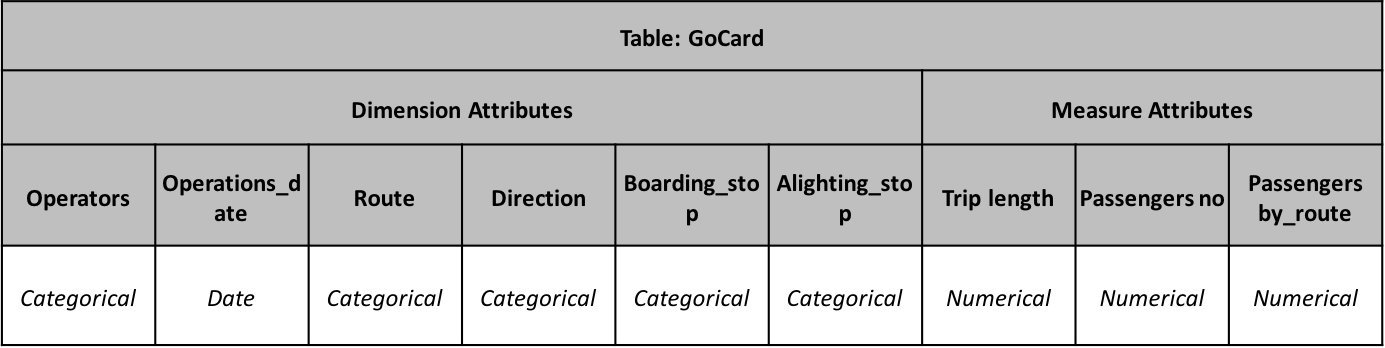
\includegraphics[width=\textwidth]{gocard_sp.png}
 	\caption{GoCard database's dimensions are classified into two: dimension attributes or measure attributes, in order to generate meaningful 2-dimensional visualization such as bar charts.}
	\label{fig:gocard_sp}
\end{figure}
%
}
%
\begin{example}
  \label{ex:gocard_sp}
 %
Using the GoCard database in Example \ref{ex:gocard}, the dimensions within that database can be classified as follows: the set of dimension attributes is $A$ = \{Operators, Operation date, Route, Boarding stop, Alighting stop, Direction\}, while the set of measure attributes is $M$ = \{trip length, passengers by route, passengers no\}, and the set of aggregate functions is $F$ = \{\texttt{count , sum , avg, max, min}\}, as shown in Figure \ref{fig:gocard_schemaandsample}.
%
Therefore, the view space of GoCard database is: $ 2 \times 6 \times 3 \times 5 = 180 $.
%
\end{example}
%
%
Though, in the context of Big Data, $SP$ is potentially a very large number. 
%
Hence, there is a need to automatically rank all these $SP$ views so that exploring them become efficient and practical.
%
To do that, each view is associated with a \emph{utility} value.
%
%
The utility of a visualization is measured as its deviation from a reference dataset $D_R$.
%
For instance, visualizations that show different trends in the query dataset (i.e. $DQ$ ) compared to a reference dataset $D_R$ are supposed to have high utility.
%
The reference dataset $D_R$ may be defined as the entire underlying dataset $D$, the complement of $DQ (D - DQ)$ 
or data selected by any arbitrary query $Q'(DQ')$.
%

Given an aggregate view $V_i$ and a probability distribution for a target view $P(V_i(DQ))$ and a reference view $P(V_i(D_R))$, the utility of $V_i$ is the distance between these two normalized probability distributions.
% 
The higher the distance between the two distributions, the more likely the visualization is to be interesting and therefore higher utility value.
%
%The utility of $U(V_i)$ is defined as the distance
%between the two normalized probability distributions of the target and comparison views.
%
Formally:
%
\begin{equation}
\label{eq:utility}
U(V_i) = S( P(V_i(DQ)), P(V_i(D)) )
\end{equation}
%
\blue{Where $S$ is a distance function (e.g., Euclidean distance, Earth Movers distance, etc). or correlation as reviewer 5 wanted.}
%\blue{it can be any type of distance function, e.g., Euclidean distance, $L_p$-norm, earth movers, etc.}
%\rply{OK}
%
Hence, the problem of visualizations recommendation is as follows \cite{DBLP:journals/pvldb/VartakMPP14}:
%
\begin{definition}
Given a user-specified query $Q$ on a database $D$, a reference dataset $D_R$, a utility function $U()$, and a positive integer $K$. 
%
Find Top-$K$ aggregate views $V_1, V_2, ..., V_K$ that have the highest utilities among all views while minimizing total computation time.
%
\end{definition}
%

Now, we are in place to present our problem statement for visualization recommendations.
%
\subsection{Problem Statement}
\label{sec:problem_statement}
%
Our proposed problem statement for visualization recommendations incorporates two limits (i.e., input parameters) to overcome the limitation of exploring all views.
%
%
\begin{definition}
\label{def:problem}
%
Given a user-specified query $Q$ on a database $D$, a reference dataset $D_R$,  a utility function $U()$, a positive integer $K$, an execution time limit $tl$ or a views number limit $R$ where $K \leq R \leq SP$.
%
Find Top-$K$ aggregate views $V \equiv (a, m, f )$ which have maximum utilities $U(V)$ among all possible views in the 
specified limits $R$ or $tl$ while maximizing the accuracy among all Top-$K$ views chosen from all $SP$ views.
%
\end{definition}
%
The limits $tl$ and $R$ in Def. \ref{def:problem} are added explicitly to overcome the limitation of exploring all views.
%
The former is a time budget that any algorithm should not exceed, while the latter is an upper bound on the number of views to be explored.
%
For instance, $tl$ can be set to zero, and $R = SP$. That is, no limit on the execution time and no limit on the number of generated views.
%
%\blue{extreme cases for $tl$ and $R$, unlimited time, $R$ equals $SP$.}
%

While those limits can be tuned by any valid value, an algorithm should output the same views as if there were no limits. 
%
This requirement makes the problem non-trivial, hence, we address it by presenting our optimization techniques encapsulated within the $RtSEngine$ framework.
%
%Next, we present our optimization techniques which address this challenge efficiently.